\documentclass[border=0.5mm]{standalone}

\usepackage{import}
\subimport{../../../}{preamble.tex}

\usepackage{tikz}
\usetikzlibrary{calc}
\usepackage{pgfplots}

\newcommand{\radiusa}{0.7}
\newcommand{\radiusb}{1.4}
\newcommand{\radiusc}{2.236}


\begin{document}

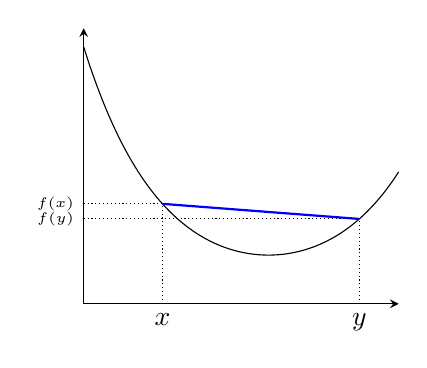
\begin{tikzpicture}

  \begin{axis}[
    ticks=none,
    axis lines=left,
    y=3.5cm,            % y unit vector
    x=1cm,            % x unit vector
    xmin=-2,
    xmax=2,
    ymin=0,
    ymax=1,
    clip=false
    ]
    
    \addplot[mark=none, black, samples=100, domain=-2:2] {(exp(-x)+exp(x)/2)/8};
    
    \addplot+[thick, draw=blue, mark=none, fill=blue] coordinates {(-1,0.362777) (1.5, 0.307996) };

    \draw[black, densely dotted] (axis cs:-1, 0) -- (axis cs:-1, 0.362777);
    \draw[black, densely dotted] (axis cs:1.5, 0) -- (axis cs:1.5, 0.307996);
    \draw[black, densely dotted] (axis cs:-2, 0.362777) -- (axis cs:-1, 0.362777);
    \draw[black, densely dotted] (axis cs:-2, 0.307996) -- (axis cs:1.5, 0.307996);

    
    \node[below] at (axis cs:-1, 0) {$x$};
    \node[below] at (axis cs:1.5, 0) {$y$};

    \node[left] at (axis cs:-2, 0.362777) {\tiny $f(x)$};
    \node[left] at (axis cs:-2, 0.307996) {\tiny $f(y)$};

    
  \end{axis}

  
\end{tikzpicture}

\end{document}

%%% Local Variables:
%%% mode: latex
%%% TeX-master: t
%%% End:
